\documentclass[11pt]{article}
%Gummi|063|=)
\title{\textbf{Data encoding for machine visualization}}
\author{Allan Inocencio de Souza Costa\\
		CloudWalk}
\date{}

\usepackage{amsmath}
\usepackage{amsfonts}
\usepackage{graphicx}
\usepackage{todonotes}
\usepackage{hyperref}
\usepackage{subfig}

\begin{document}

\maketitle

\section{Introduction}

This document is just a informal report of some experiments realized in search of a procedure that could generate images from raw data, but with some constraints. 

\subsection{Justification}

We want to generate distinct images representing distinct classes from arbitrary datasets. We could use those images to train a semi-supervised classifier, meaning that we could train a Convolutional Neural Network (CNN) to learn features from those images and later we could use these features to train a softmax classifier with little labeled data. We are also interested in pure unsupervised methods, so one approach would be to compute a similarity score for those images, which could be easily done given the great amount of works in that subject found in the literature, leaving us with a complete unsupervised system. Another approach would be to use some unsupervised clustering algorithm in top of the features learned from the images, giving us a previously fixed number of data clusters sharing some degree of similarity within each of them. We could afterwards compare these kind of system with some standard clustering algorithms. Finally, maybe we could try something along \href{http://arxiv.org/pdf/1112.6209.pdf}{Google's research paper on unsupervised learning}, in which we could try to pick up the most responsive output neuron in a deep\footnote{We need some depth not because our images are too complex, but because we need high level abstractions from them.} (convolutional or non-convolutional) neural network and see if its activation has some correlation within diffeerent clusters (classes). 

For this report we used only supervised learning, as the classification accuracy is a good metric for how well our encoders perform and as it has a direct efficient implementation in Caffe framework.

\subsection{Overview}

Considering classification tasks with machine learning, our main ideia is that if we could generate distinguishable images from data points in different classes, we could train a CNN to pick the right class of a given data point. 

For the sake of clearness, let $\mathbf{x} = (x_1, x_2, \dots, x_m) \in \mathbb{R}^m$ be a $m$-dimensional vector holding our original data point (so we have $m$ features). What we want is a function $f: \mathbb{R}^m \rightarrow I$, that takes a data point $\mathbf{x}$ and outputs an image $f(\mathbf{x})$. Such a function $f$ must be constrained having our goals in mind. As an example, it won't work to just project the points in different planes and then overlap them.

Being a machine learning project, we are insterested in patterns within data, so our main constraint is that we want to generate images that looks similar for similar inputs, but distinct for unalike inputs. Using the classification community jargon, we want images that belong to the same class to be similar between them, but different from images of another class. Related to this, if we produce continuous deformations of the input, we want continous deformations of the input. Said another way, if we change $x_1 = 0.99$ to $x_1 = 1.00$, while mantaining the other features unchanged, we want the output image to change slightly.

Our methodology was empirical. We used some labeled datasets to prototype good (to our eyes) encoders in Mathematica. After that we used Caffe for a CNN implementation, which receives the data encoded as images as input and tests our encoder capability by classifying the images into predicted classes. We also used scikit-learn to train standard classifiers for the datasets we used, so that we could compare our method with more standard ones. The classifiers used were GNB (Gaussian Naive Bayes), RF (Random Forests), SVM (Support Vector Machine) and KNN (k-Nearest Neighbors).

All the code is available in the repository \href{www.github.io/allanino/data-encoding}{www.github.io/allanino/data-encoding}.

\section{Datasets} \label{sec:datasets}

In this section we provide a brief description and motivation for each dataset we used so far. The main information is in table \ref{table:datasets}.

\begin{table}[htp]
\centering
\begin{tabular}{|c|ccc|}
\hline
	Dataset & Train size & Test size & Number of classes\\ \hline
	Iris & 120 & 30 & 3\\
	Leaf & 268 & 72 & 30\\
	Titanic & 1760 & 441 & 2\\
\hline
\end{tabular}
\caption{Datasets information. We always have a $80\%$-$20\%$ split for train and test.}
\label{table:datasets}
\end{table}


\subsection{Iris}
The  \href{http://archive.ics.uci.edu/ml/datasets/Iris}{Iris dataset} is the first dataset we considered using given its simplicity and highly data separability. It consists of $150$ data points with $4$ features each. The features are measures of flowers of the $Iris$ species. We have measures of petals and sepals width and length for $3$ classes of flowers: \emph{Iris setosa}, \emph{Iris virginica} and \emph{Iris versicolor}.

\subsection{Leaf}

After we achieved satisfatory results with the Iris dataset, we aimed at a more challenging dataset, in order to validate our results. We found the \href{http://archive.ics.uci.edu/ml/datasets/Leaf}{Leaf dataset}, but maybe it was too challenging, for it have too many classes ($30$ leaf species) and too few data points ($340$), which we still have to split between training and testing sets. It have many more features ($14$), all real valued, with large scale variation. Nonetheless, we still could achieve some decent results (much better than baseline), and it was a good validator for our enconding methods, as it allowed us to see a great variety of images.

\subsection{Titanic}

After our experiments with the Leaf dataset, we aimed at the other extreme and found the \href{http://sci2s.ugr.es/keel/dataset.php?cod=189}{Titanic dataset}, which is suited for a binary classification task (to predict wheter a given passenger survived or not). The data has $3$ features: passenger sex, age and social class, encoded as real numbers (how the encoding was done is unclear from the source, but it does not matter,as we are using other classification algorithms as comparisson). With its $2201$ data points, we have a lot of examples to train our CNN.

\section{Encoders} \label{sec:encoders}

We have tested some encoders, but we will focus on the best ones. I will use the names of the functions we created in Mathematica for them.

\subsection{PermutationEncoder}
This one was our first ideia: we permutate the features in groups of 2, obtaining a lot of pairs of points (exactly $m(m-1)$). We then join the points sequentialy to form a polygon. As sides of the polygon can cross each other, we have to paint its interior in a way that reflects the crossing, but it is done automatically by Mathematica's \textsc{Polygon} function, which paints the closed areas while avoiding to paint adjacent areas.

\textbf{Example:} Consider the following data point from Iris:
\[
\mathbf{x} = (6.4,3.2,4.5,1.5)
\]

The sequence of permutated points is given as following:
\[
P = 
\left(
\begin{array}{cc}
 6.4 & 3.2 \\
 6.4 & 4.5 \\
 6.4 & 1.5 \\
 3.2 & 6.4 \\
 3.2 & 4.5 \\
 3.2 & 1.5 \\
 4.5 & 6.4 \\
 4.5 & 3.2 \\
 4.5 & 1.5 \\
 1.5 & 6.4 \\
 1.5 & 3.2 \\
 1.5 & 4.5 \\
\end{array}
\right)
\]

Now we plot these points in a two dimensional space, joining consecutive ones, as in figure \ref{fig:P} a). Observe that the last point is joined to the first one. Finally, we paint closed regions, but keeping adjacent ones with different color, as in figure \ref{fig:P} b).

\begin{figure}[htp]
    \centering
    \subfloat[Joining the points.]{{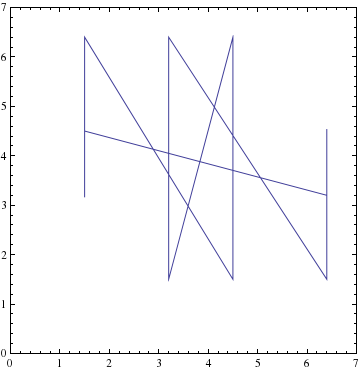
\includegraphics[scale=0.45]{permutationPlot.png} }}
    \qquad
    \subfloat[Painting interiors.]{{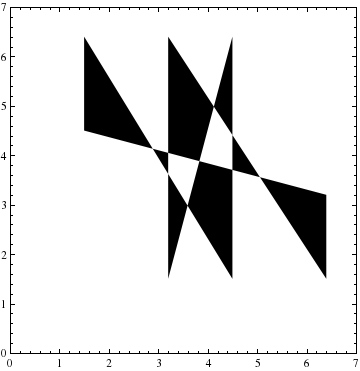
\includegraphics[scale=0.45]{permutationGraph.png} }}
    \caption{Creating the image from the permutaions.}
    \label{fig:P}
\end{figure}

\subsection{SubsetEncoder}
This encoding is similar to \textsc{PermutationEncoder} in every steps but one: we don't take all the permutation pairs, but only those that don't repeat the same two features. For instance, if we use choose to use the pair $(x_1,x_2)$ we don't use $(x_2,x_1)$. The motivation for it was the Leaf dataset great number of features, which produces a polygon of $14*13 = 182$ vertices under the \textsc{PermutationEncoder}.

\textbf{Example:} Consider the following data point from Iris:
\[
\mathbf{x} = (6.4,3.2,4.5,1.5)
\]

The sequence of subsets with 2 points is given as following:
\[
P = 
\left(
\begin{array}{cc}
 6.4 & 3.2 \\
 6.4 & 4.5 \\
 6.4 & 1.5 \\
 3.2 & 4.5 \\
 3.2 & 1.5 \\
 4.5 & 1.5 \\
\end{array}
\right)
\]

From here we follow as in the previous section. The results are in figure \ref{fig:S}.

\begin{figure}[htp]
    \centering
    \subfloat[Joining the points.]{{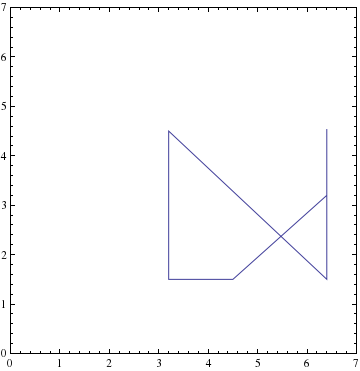
\includegraphics[scale=0.45]{subsetPlot.png} }}
    \qquad
    \subfloat[Painting interiors.]{{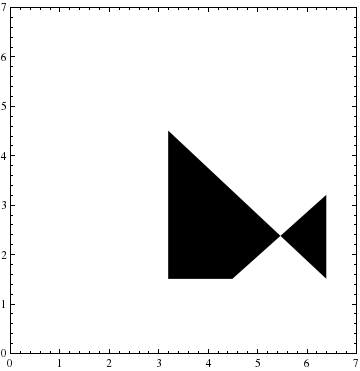
\includegraphics[scale=0.45]{subsetGraph.png} }}
    \caption{Creating the image from the subsets.}
    \label{fig:S}
\end{figure}

\subsection{RadarEncoder}

Here we use a kind of radar plot. We take a circle of radius $r = 1$ and divide it in $m = \text{number of features}$ points, marking, in effect, the vertices of a $m$ sided regular polygon. The ideia is to plot the value of each feature in the direction from the center to the respective feature vertex and with distance to the center proportional to its numerical value (its absolute value). The main drawback with this encoding is that we need prior information about the minimum and maximum value of each feature so that we can rescale it to the $[0,1]$ range, as $1$ is the maximum distance from the center allowed by our encoding. After we join these points, forming a polygon.


\textbf{Example:} Consider the following data point from Iris:
\[
\mathbf{x} = (6.4,3.2,4.5,1.5)
\]
As we have four features, our resulting points would lie in the direction of four vertex forming a square. The vectors with the maximum and minimum values of each feature, for the Iris dataset, are:
\[
\mathbf{x_{max}} = (7.9, 4.4, 6.9, 2.5)
\]
\[
\mathbf{x_{min}} = (4.3, 2.0, 1.0, 0.1)
\]
So the rescaled version of our original data point, alread taken its module, is:
\[
\bar{\mathbf{x}} = (0.417, 0.500, 0.407, 0.417)
\]

To find the position of the point that refers to the $k$-th feature, we multiply the corresponding coordinate of $\bar{\mathbf{x}}$ by the unitary vector in the wanted direction:
\[
P_k = \bar{x}_k \cdot \left( \cos \left( \frac{2\pi k}{m} \right), \sin \left( \frac{2\pi k}{m} \right) \right ) = \bar{x}_k \cdot \left( \cos \left( \frac{2\pi k}{4} \right), \sin \left( \frac{2\pi k}{4} \right ) \right )
\] 

Working that way for $k = 0,1,2,3$, we obtain four points that we can then join to form a polygon, as shown in figure \ref{fig:R}.

\begin{figure}[htp]
\centering
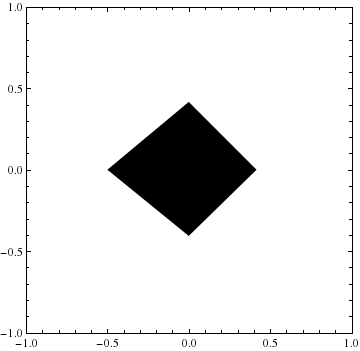
\includegraphics[scale=0.65]{radarGraph.png}
\caption{A \textsc{RadarEncoder} example.}
\label{fig:R}
\end{figure}

\subsection{TextEncoder}
This one must be the most unusual of all, in that we simple let our CNN ``see'' the raw data. This encoder simple concatenates the sign ($+$ or $-$) of each feature with its two most significant digits and the number of digits to the left of the decimal point, putting each string so concatenated in a grid, i.e., each image contain the raw numerical information of the data point. It may look silly, but it worked well in practice.

\textbf{Example:} Consider the following bogus data point:
\[
\mathbf{x} = (6.4,0.32, -47.5,0.00015)
\]

Following the above instructions, we have the following correspondence:
\begin{align*}
6.4 &\mapsto \text{+64+1} \\
0.32 &\mapsto \text{+32+0} \\
-47.5 &\mapsto \text{-47+2} \\
0.00015 &\mapsto \text{+15-3}
\end{align*}

The resulting image is in figure \ref{fig:T}.

\begin{figure}[htp]
\centering
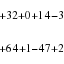
\includegraphics[scale=1.0]{text.png}
\caption{A \textsc{TextEncoder} example.}
\label{fig:T}
\end{figure}

\section{Results}

Here we discuss in detail the results of our experiments with each encoder of section \ref{sec:encoders} in each dataset of section \ref{sec:datasets}. For each dataset, we trained four models in sklearn (GNB, RF, SVM, KNN) 50 times each, taking the mean of the 50 accuracies as the accuracy of each model. In each run of each model we randomly split our dataset in $80\%$ training and $20\%$ test\footnote{A better methodoly would be to use the same 50 splittings for each model, but our methodoly was easier to implement and is good enough for our purposes.}. We also trained a CNN 50 times for each dataset and each type of encoder.  

\subsection{Iris}
In this dataset, our encodings performed systematically worse than the traditional approaches. See table \ref{table:iris} below for the results.

\begin{table}[htp]
\centering
\begin{tabular}{|c|c|}
\hline
	Model & Accuracy \\ \hline
	GNB & 0.949\\
	\textbf{RF} & \textbf{0.983} \\
	SVM & 0.977\\
	KNN & 0.977\\
	CNN (\textsc{PermutationEncoder}) & 0.953 \\
	CNN (\textsc{TextEncoder}) & 0.931 \\
\hline
\end{tabular}
\caption{Iris results.}
\label{table:iris}
\end{table}

As you can see, our encoders plus a CNN performed more or less similarly to the conventional methods. Here you can confirm our previous claim about the good performance of the \textsc{TextEncoder}.

\subsection{Leaf}
These are our worse results, but other distance based methods performed poorly as  well, as you we can see from table \ref{table:leaf}.

\begin{table}[htp]
\centering
\begin{tabular}{|c|c|}
\hline
	Model & Accuracy \\ \hline
	GNB & 0.775\\
	\textbf{RF} & \textbf{0.864} \\
	SVM & 0.223\\
	KNN & 0.601 \\
	CNN (\textsc{RadarEncoder}) & 0.734 \\
	CNN (\textsc{ColorRadarEncoder}) & 0.746 \\
	CNN (\textsc{SubsetEncoder}) & 0.567 \\
	CNN (\textsc{TextEncoder}) & 0.443 \\
\hline
\end{tabular}
\caption{Leaf results.}
\label{table:leaf}
\end{table}

In this dataset our best encoder was the \textsc{RadarEncoder}. We could not achieve a better result, despite a lot of effort put into it. Maybe the great performance of Random Forests can give a hint of why, as it is an ensemble method, in our case it is averaged out of 200 estimators.  The \textsc{TextEncoder} performed rather poorly here\footnote{The average reported was taken from just 10 data partitions, as we needed a lot more training here, given the fine structure of our images.}, but this is not so surprising, given that our text had to be smaller and our image larger to contain the data of all $14$ features. Even so, its performance is much better than random guess ($3.33\%$).

\subsection{Titanic}
This dataset has the most interesting results. The accuracies of each model are on table \ref{table:titanic}.


\begin{table}[htp]
\centering
\begin{tabular}{|c|c|}
\hline
	Model & Accuracy \\ \hline
	GNB & 0.774\\
	RF & 0.789 \\
	\textbf{SVM} & \textbf{0.791}\\
	KNN & 0.758 \\
	CNN (\textsc{PermutationEncoder}) & 0.771 \\
	CNN (\textsc{TextEncoder}) & 0.782 \\
\hline
\end{tabular}
\caption{Titanic results.}
\label{table:titanic}
\end{table}

In this dataset all performances was similar. But we would like to point out the \textsc{TextEncoder} good performance. 

\section{Partial conclusion}
There are some lesson we could take from the above results. The first one is that our results from different encoding methods are pretty similar. The second lesson is that our results with CNNs are similar to more standard methods. The third one is that even a straightforward encoding like our \textsc{TextEncoder} is capable of good results.

Now, maybe lesson one can teach us even more if we ask: Why we got consistently similar results for different image encoders? It could be because we always used the same CNN design, but this a poor explanation, for we did experiments with discontinous encoders that performed better than baseline (random guess), but worse than our more well-behaved encoders. We propose the following explanation: we can't take water from dry stones. The meaning of this is that we can't get more information than what the data gives us, and this implies that there is a limit to the accuracy of whatever method we use. This is well ilustrated with the Titanic dataset, as we have lots of overlaping points\footnote{We have a lot of points with identical features, but members of diffent classes. In this context, that can be interpreted as passengers that died even being wealth womans with kids, for example.}. So the better models are the ones whose accuracy gets closest to this fundamental maximum.

An important question is whether our CNN architecture is the best choice. It has 3 convolutional layers (with  pooling and ReLu) plus 2 fully connected layers followed by a softmax layer. What if it has too many parameters, being prone to overfitting? Or perhaps that is not the problem, but it is too shallow (this is less probable, as it was good enough to give great results in Cifar-10 dataset, which contains much more diverse images).
So future experiments could try different architectures. But we argue that the architecture used is good enough in capturing geometric details of images, as it is can distinguish images of one class or another if they are distinct enough to humans tell one type from another. Even more, it can see patterns were we struggle to do so, as was proven by the unlikely (at first) good performance of the \textsc{TextEncoder}.

One final word about the pratical use of it as a classifier. In the datasets we tested, the Random Forest algorithm performed well enough to justify its use instead of our new schema (even more if we remember it is less computational expensive). But it has to be retrained if new classes join the dataset, while our algorithm would have only to retrain the softmax weigths. Given the way Decision Trees work, splitting the data according the information content of each feature, and the way Random Forest works, creating multiple Decision Trees from random samples of the dataset, maybe we could use a similar approach in our encoding system, i.e., we could try to put in some information theoretical stuff, the most obvious being entropy, but I really want to avoid using a priori information about classes (an ideal encoding woulld have that information hidden in it anyway).
\end{document}
